\documentclass{article}
\usepackage{graphicx}  % To include images
\usepackage{booktabs}  % For better table formatting
\usepackage{amsmath}
\usepackage{booktabs}
\usepackage[export]{adjustbox}

% Define the \sym command for significance levels
\newcommand{\sym}[1]{%
  \ifmmode^{#1}\else\(^{#1}\)\fi%
}
\begin{document}
\title{Randomization assessment}
\author{Riccardo D.C.}
\date{21 September 2023}
\maketitle
\section{Traditional method}
\begin{table}[htbp]
    \centering
    \caption{Differences in means across Maropitant and Metadone}
    \begin{tabular}{ccc}
        \begin{tabular}{l*{3}{c}}
            \hline\hline
                        &     &            &            \\
                        &Metadone(control)&Maropitant(treatment)&     p-value\\
            \hline
            Age         &        15.9&       16.95&    .4321982\\
            Weight      &       19.95&       20.85&    .2792915\\
            \hline\hline
        \end{tabular}
            
    \end{tabular}
\end{table}
The table displays the means of two key variables, 'Age' and 'Weight,' stratified by treatment status. The p-values in
the last column correspond to the results of t-tests comparing the means of these variables between the treatment and
control groups. \\
\par
Notably, the p-values for both 'Age' and 'Weight' are relatively large, with 'Age' yielding a p-value of approximately
0.4322 and 'Weight' yielding a p-value of around 0.2793. These large p-values are indicative of the success of the
randomization process. In the context of this experiment, larger p-values suggest that there are no statistically
significant differences in these key characteristics between the treatment and control groups. This reinforces our
confidence in the randomization process, indicating that it effectively balanced these variables across the two groups,
thereby enhancing the validity of our experimental findings.
\begin{table}[!h]\centering
    \def\sym#1{\ifmmode^{#1}\else\(^{#1}\)\fi}
    \caption{Regression probit to check randomization}
    \begin{tabular}{l*{1}{c}}
    \toprule
     
                        &\multicolumn{1}{c}{Maropitant}\\
    \midrule
        &                     \\
    Age                 &       0.045         \\
                        &     (0.050)         \\
    \addlinespace
    Weight                &       0.094         \\
                        &     (0.080)         \\
    \addlinespace
    Constant            &      -2.662         \\
                        &     (1.915)         \\
    \midrule
    Observations        &          40         \\
    LR chi2(2)          &      2.07             \\
    Prob > chi2         &   0.3549              \\

    \bottomrule
    \multicolumn{2}{l}{\footnotesize Standard errors in parentheses}\\
    \multicolumn{2}{l}{\footnotesize  }\\
    \multicolumn{2}{l}{\footnotesize \sym{*} \(p<0.10\), \sym{**} \(p<0.05\), \sym{***} \(p<0.01\)}\\
    \end{tabular}
\end{table}
    
The results of the probit regression provide important evidence supporting the success of our randomization process. The
coefficient estimates for 'Age' and 'Weight,' which represent potential confounding variables, do not show statistically
significant relationships with the treatment variable 'Maropitant.' Additionally, the likelihood ratio (LR) chi-squared
test, which assesses the overall significance of the covariates, yields a p-value of 0.3549, indicating that these
covariates collectively do not significantly predict the treatment assignment. This suggests that the randomization
process effectively balanced these characteristics between the treatment and control groups, reinforcing our confidence
in the experiment's validity. 

\subsection{Plots}
\begin{figure}[!h]
\centering
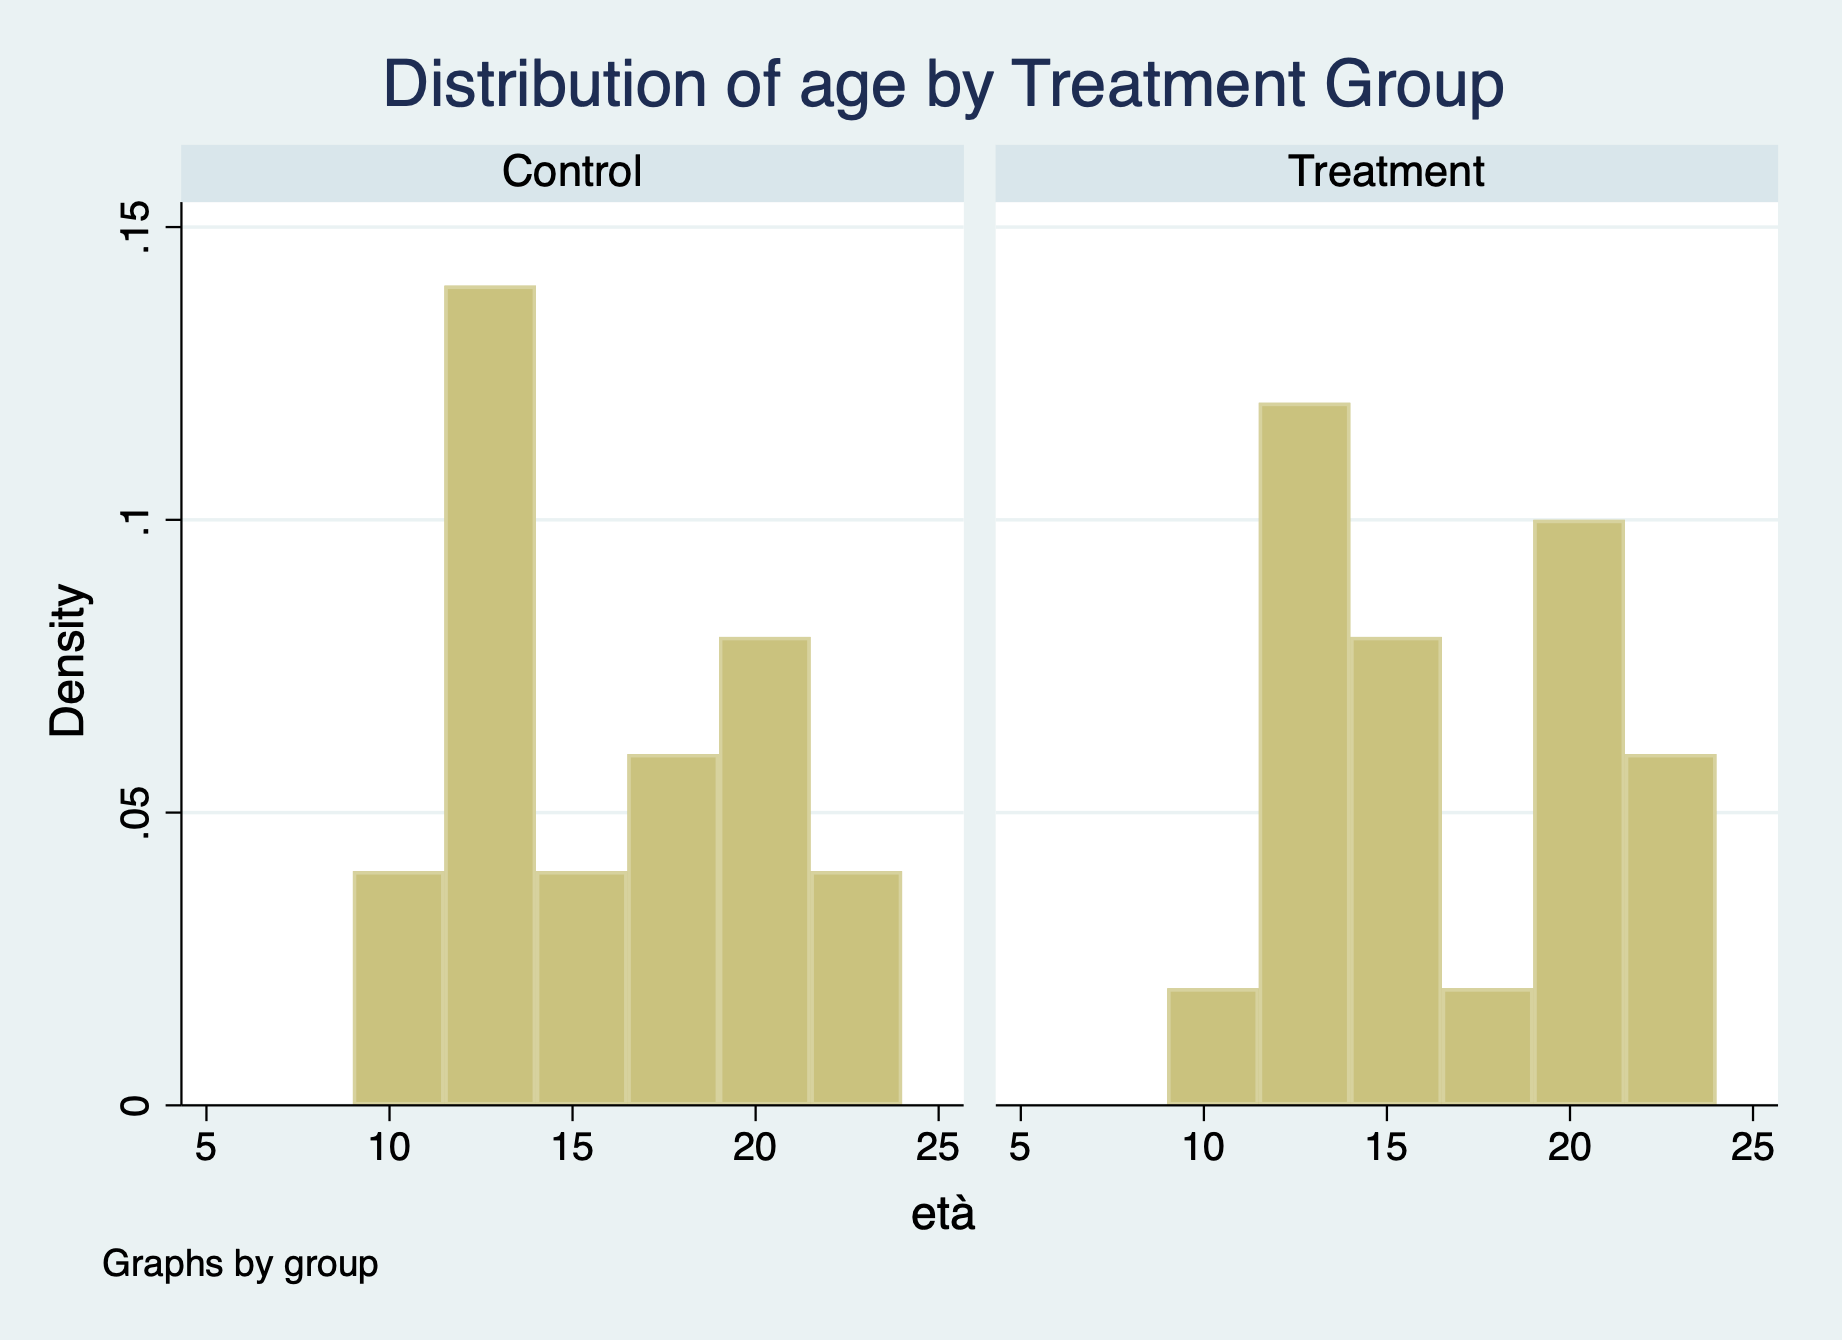
\includegraphics[scale=0.30]{histogram_eta_trad.png}
\caption{Histogram of age by Treatment Group}
\end{figure}

\begin{figure}[!h]
\centering
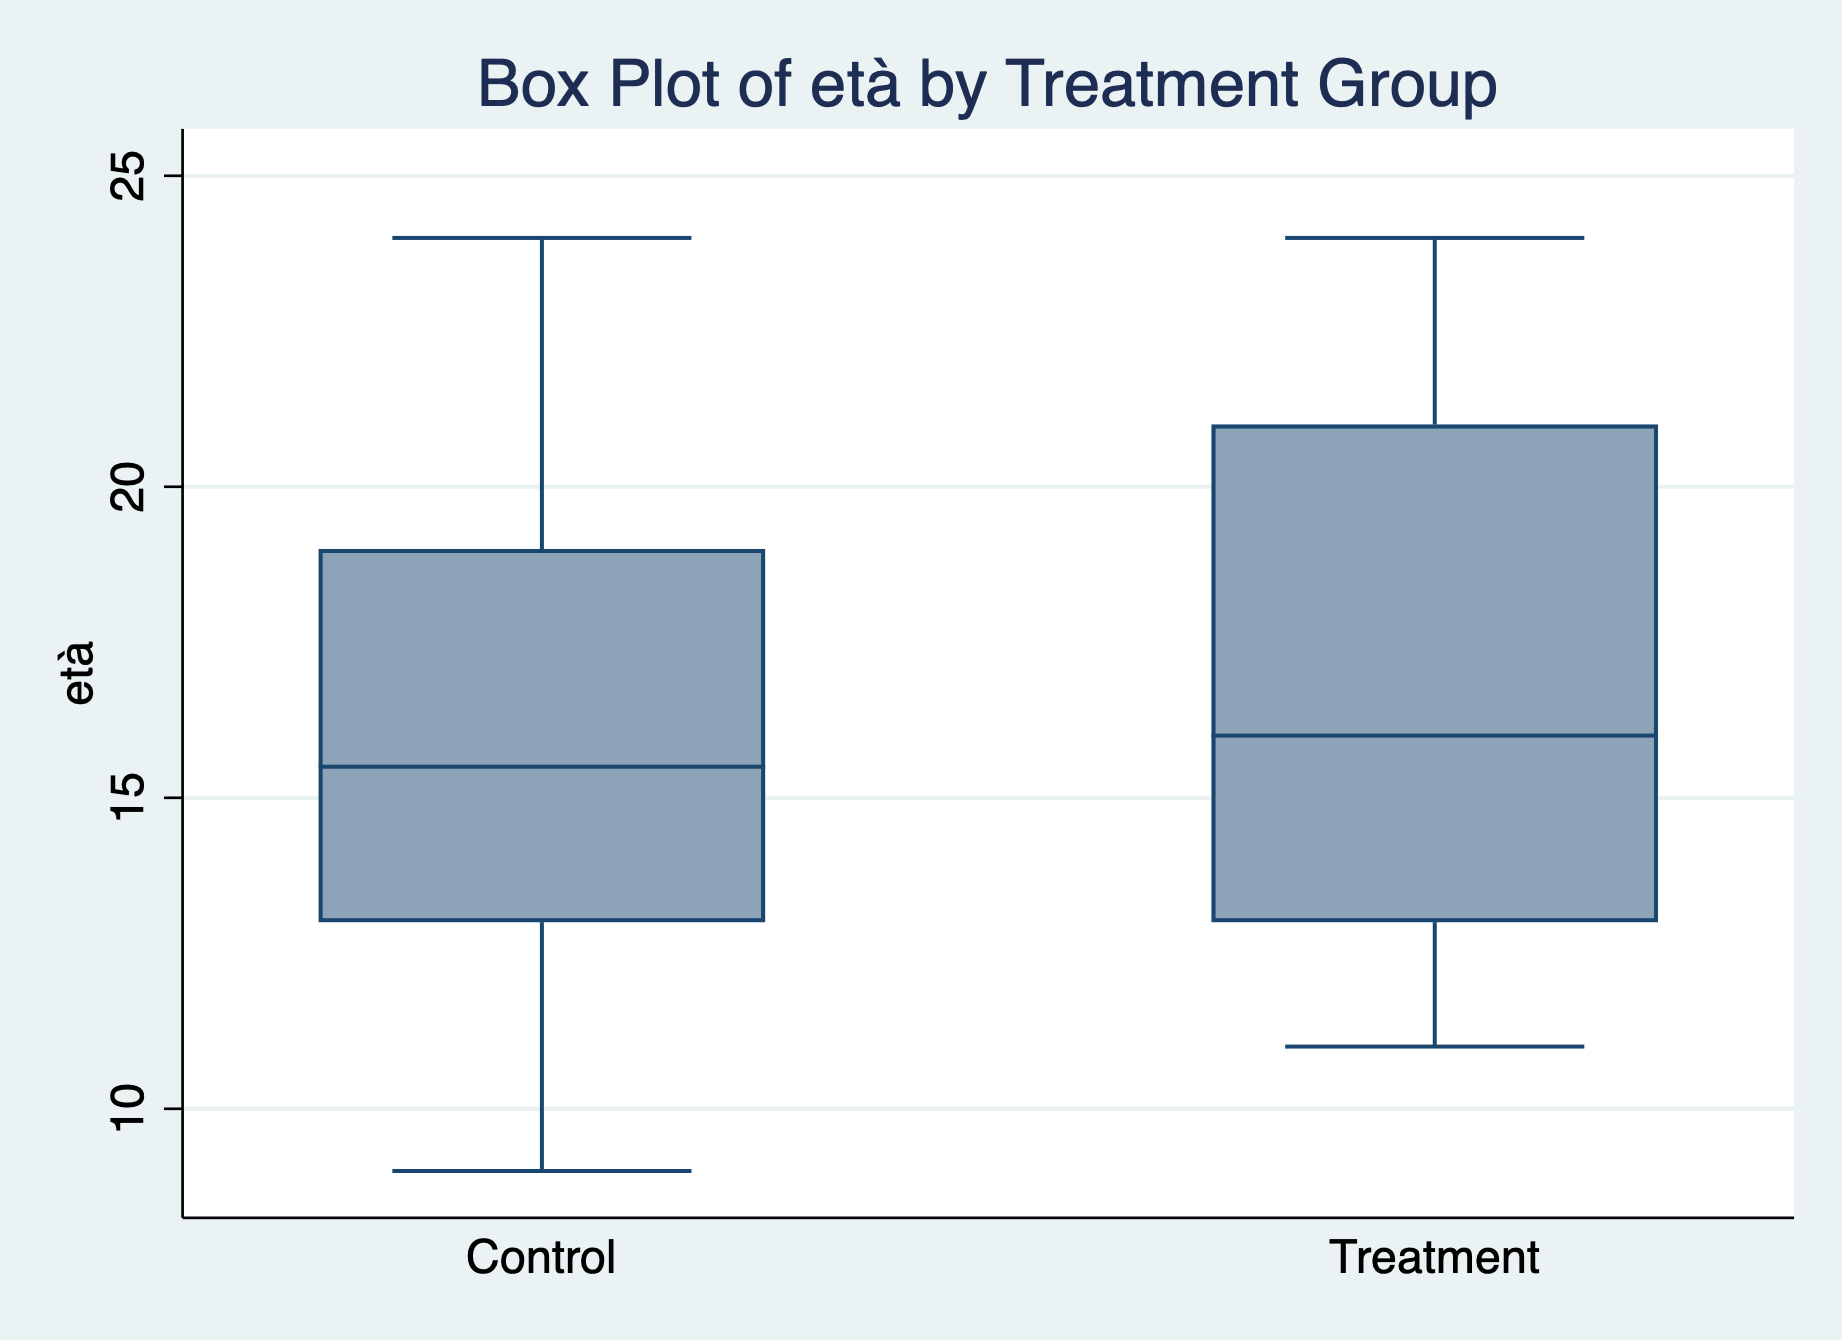
\includegraphics[scale=0.30]{box_plot_eta_trad.png}
\caption{Box Plot of age by Treatment Group}
\end{figure}

\begin{figure}[!h]
\centering
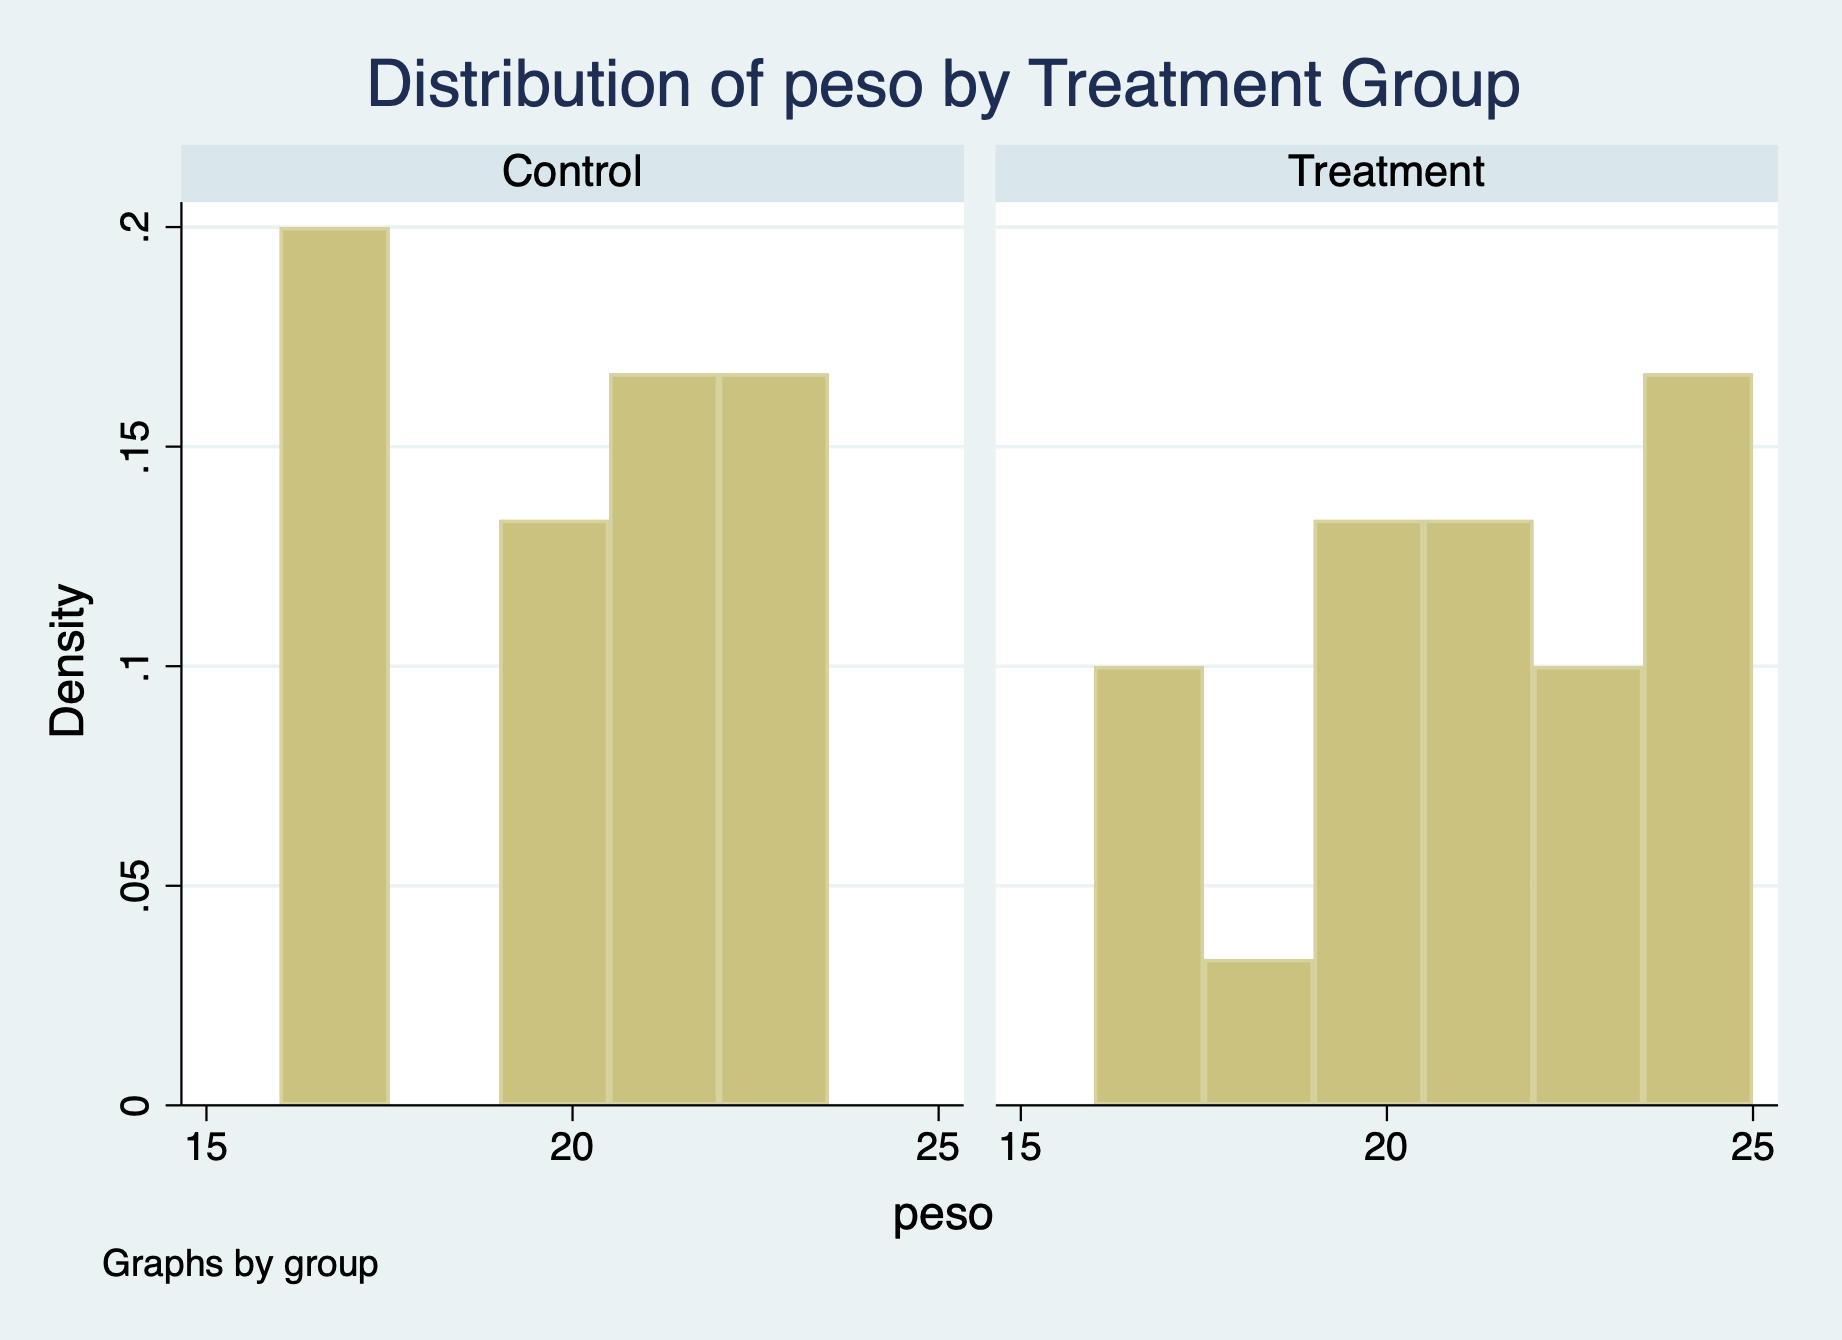
\includegraphics[scale=0.30]{histogram_peso_trad.png}
\caption{Histogram of weight by Treatment Group}
\end{figure}

\begin{figure}[!h]
\centering
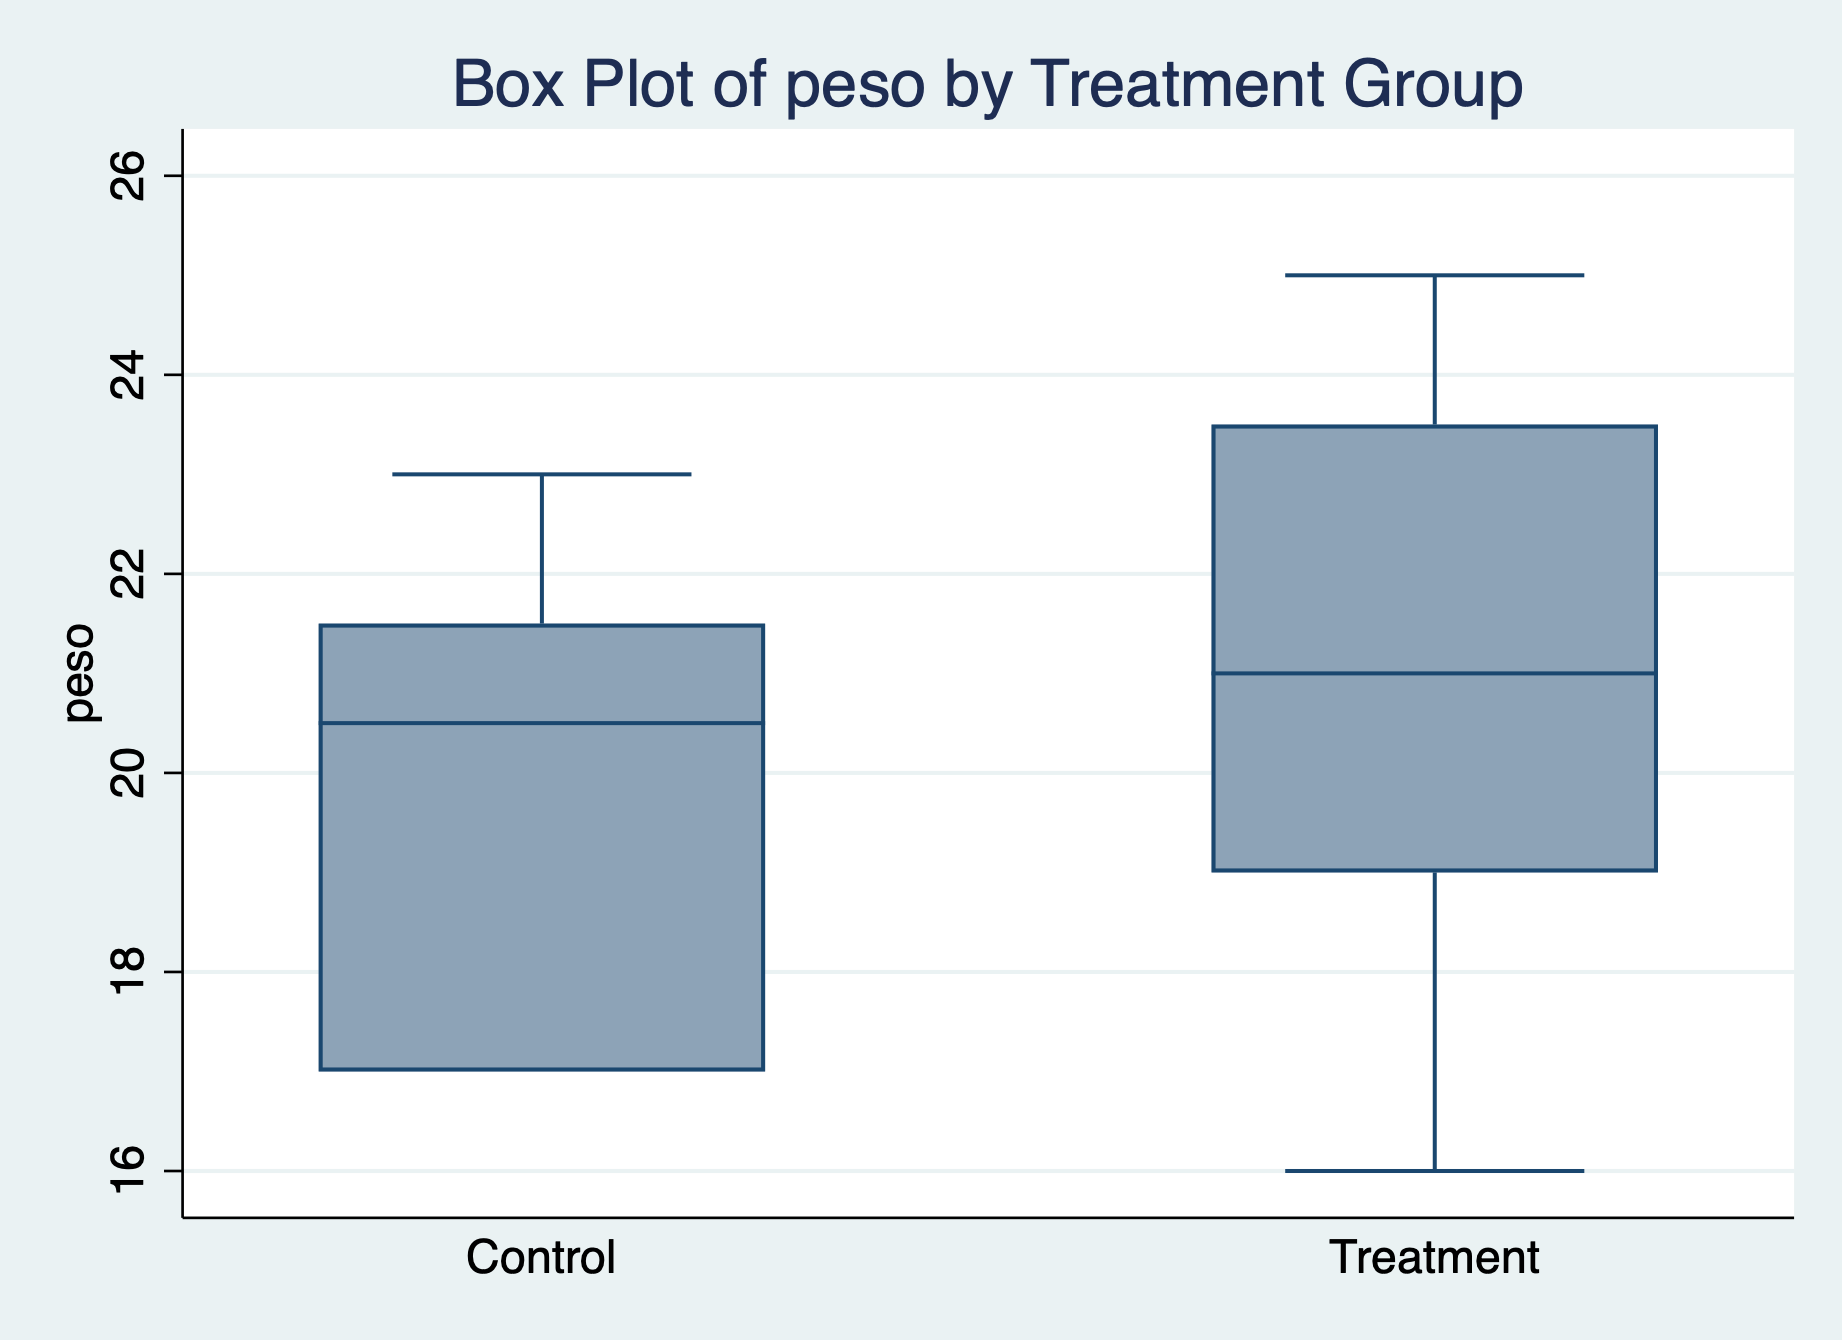
\includegraphics[scale=0.30]{box_plot_peso_trad.png}
\caption{Box Plot of weight by Treatment Group}
\end{figure}

Investigating the randomization success of our experiment, we turn our attention to the provided plots. These visual
representations showcase the distribution of key variables among the treatment and control groups. Notably, the plots
reveal a striking similarity in the distribution of variables between the two groups, with substantial overlap observed.
This alignment suggests that the randomization process effectively balanced the covariates, ensuring that both groups
exhibit comparable characteristics. The absence of pronounced differences between the treatment and control groups in
these plots reinforces our confidence in the validity of the randomization procedure, strengthening the foundation upon
which our experimental conclusions are built. 
\section{Thunder method}
\begin{table}[htbp]
    \centering
    \caption{Mean Values by Treatment Group (Thunder Method)}
    \begin{tabular}{l*{3}{c}}
    \hline\hline
                & Metadone (control) & Maropitant (treatment) & p-value \\
    \hline
    Age         & 15.05 & 16.00 & 0.4516 \\
    Weight      & 19.00 & 20.00 & 0.2429 \\
    \hline\hline
    \end{tabular}
\end{table}
The table presents the means of two key variables, 'Age' and 'Weight,' categorized by treatment group. The p-values in
the last column represent the outcomes of t-tests that compare the means of these variables between the treatment and
control groups. \\
\par
Notably, the p-values for both 'Age' and 'Weight' are relatively large, with 'Age' yielding a p-value of approximately
0.4516 and 'Weight' yielding a p-value of approximately 0.2429. These sizable p-values serve as strong evidence in favor
of the successful implementation of the randomization process. Within the context of this experiment, larger p-values
suggest that there are no statistically significant disparities in these crucial characteristics between the treatment
and control groups. This reaffirms our confidence in the effectiveness of the randomization process, as it has
effectively balanced these variables between the two groups, thereby bolstering the credibility of our experimental
results. 
\begin{table}[htbp]
    \centering
    \caption{Probit Regression to Check Randomization}
    \begin{tabular}{l*{1}{c}}
        \toprule
                            &\\
                            &\multicolumn{1}{c}{Maropitant}\\
        \midrule
                &                     \\
        Age                 & 0.048               \\
                            & (0.053)             \\
        \addlinespace
        Weight              & 0.100               \\
                            & (0.078)             \\
        \addlinespace
        Constant            & -2.682              \\
                            & (1.836)             \\
        \midrule
        Observations        & 40                  \\
        LR chi2(2)          &      2.27             \\
        Prob > chi2         &   0.3220              \\
        \bottomrule
        \multicolumn{2}{l}{\footnotesize Standard errors in parentheses}\\
        \multicolumn{2}{l}{\footnotesize  }\\
        \multicolumn{2}{l}{\footnotesize \sym{*} \(p<0.10\), \sym{**} \(p<0.05\), \sym{***} \(p<0.01\)}\\
    \end{tabular}
\end{table}
    
The results of the probit regression provide important evidence supporting the success of our randomization process.
The coefficient estimates for 'Age' and 'Weight,' which represent potential confounding variables, do not show
statistically significant relationships with the treatment variable 'Maropitant.' Additionally, the likelihood ratio
(LR) chi-squared test, which assesses the overall significance of the covariates, yields a p-value of 0.3549,
indicating that these covariates collectively do not significantly predict the treatment assignment. This suggests
that the randomization process effectively balanced these characteristics between the treatment and control groups,
reinforcing our confidence in the experiment's validity.
    



\subsection{Plots}

\begin{figure}[h]
\centering
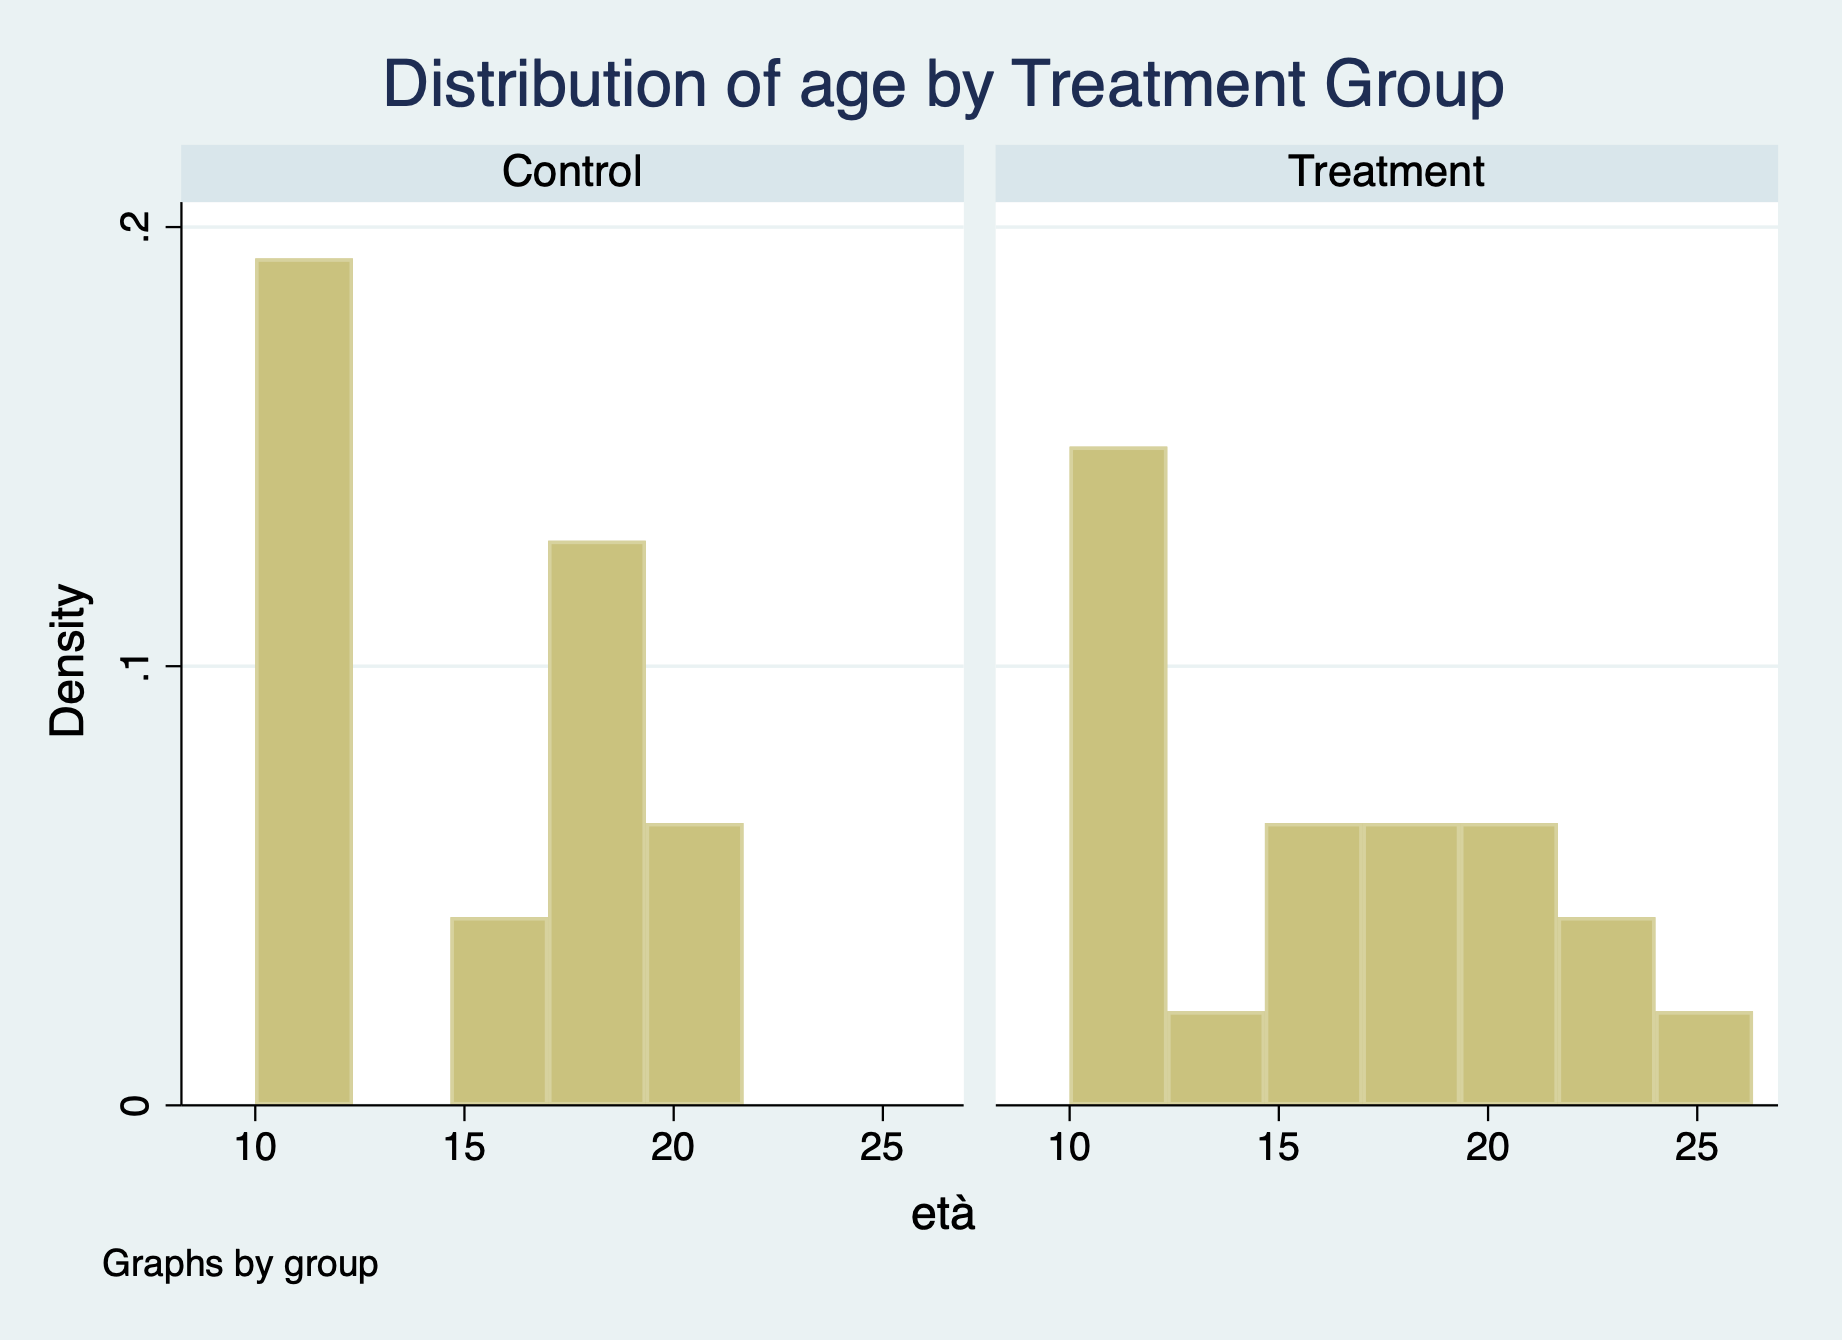
\includegraphics[scale=0.30]{histogram_eta_ntrad.png}
\caption{Histogram of age by Treatment Group}
\end{figure}

\begin{figure}[h]
\centering
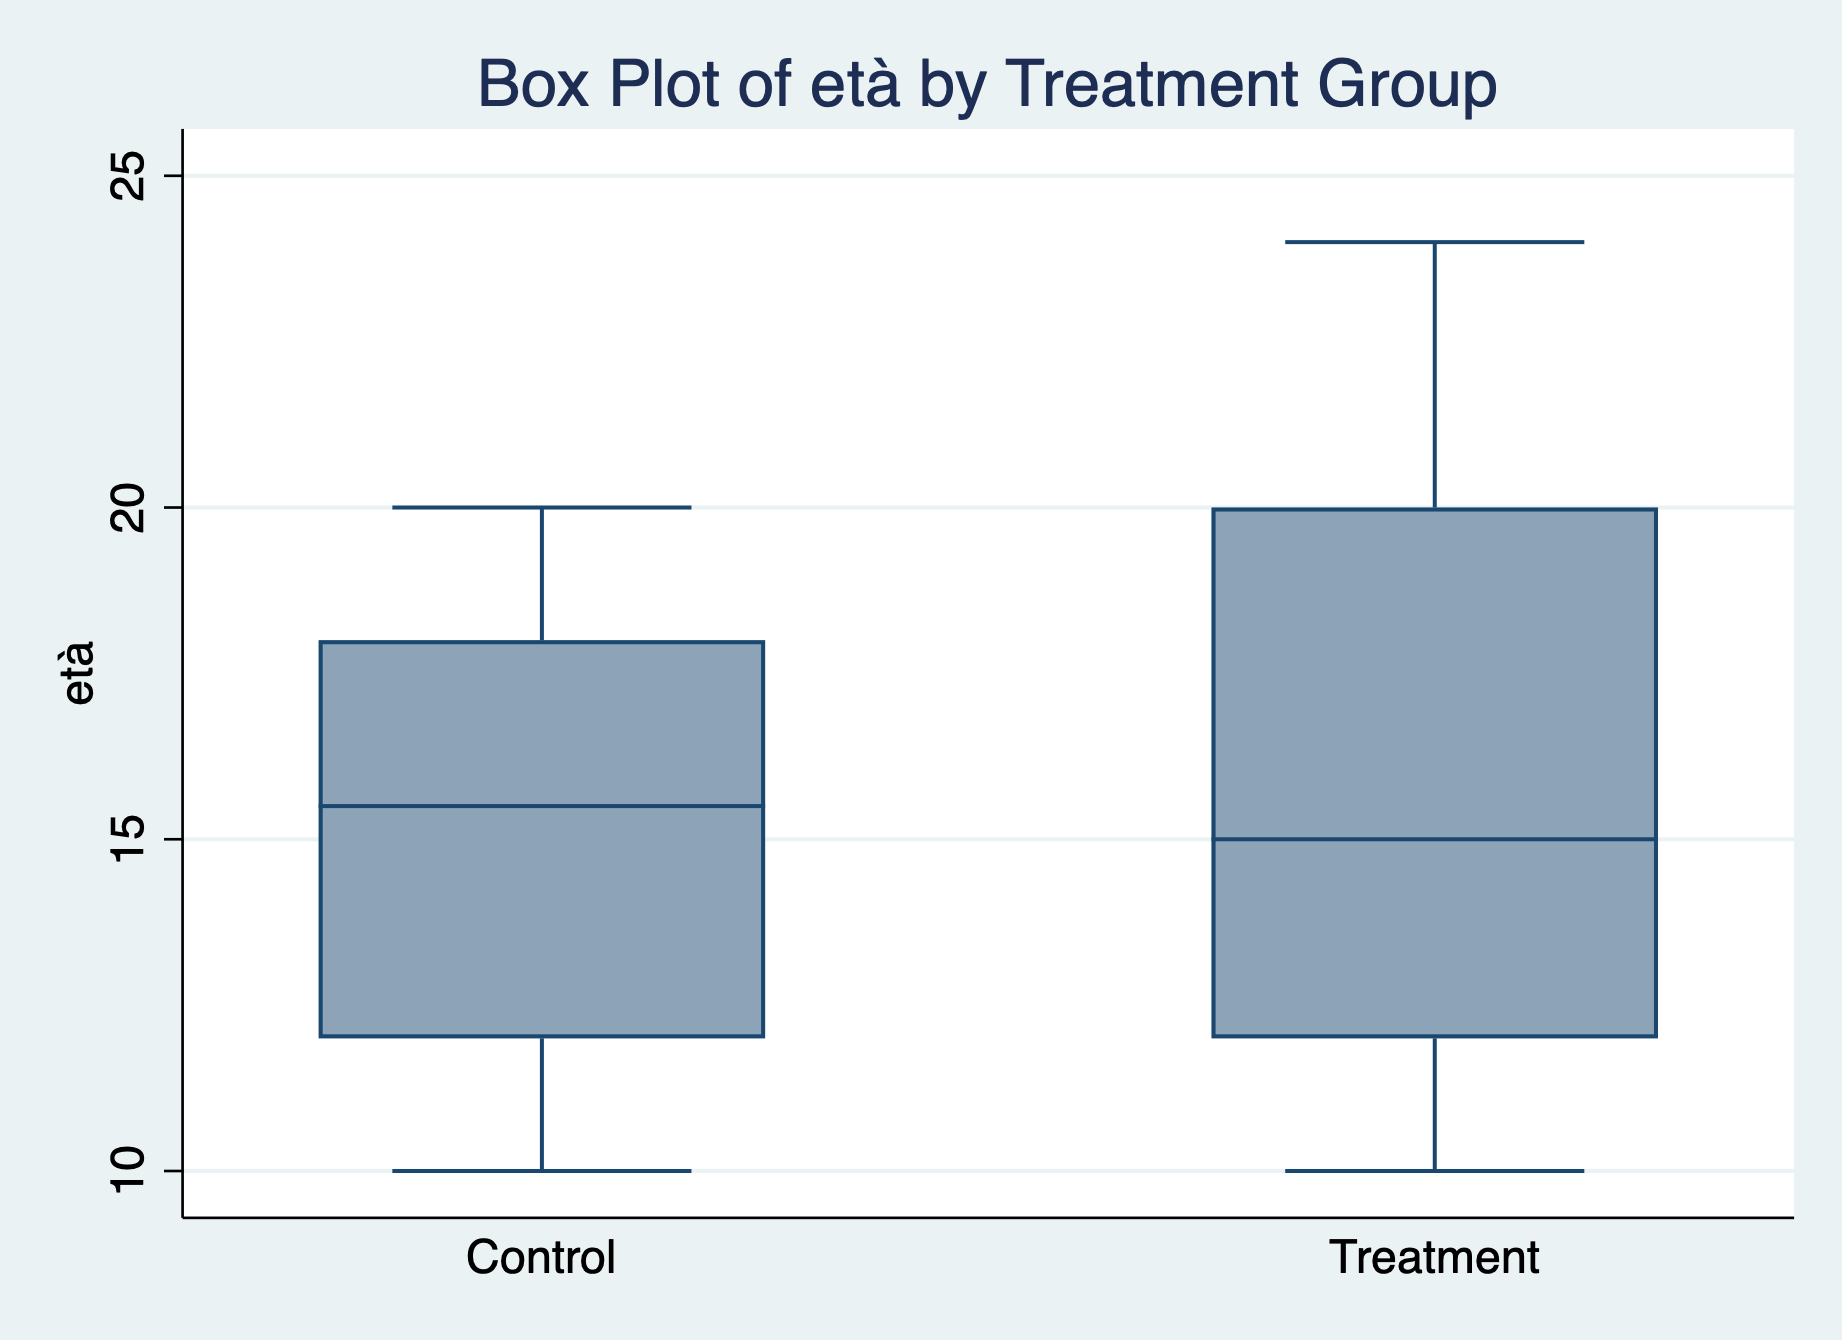
\includegraphics[scale=0.30]{box_plot_eta_ntrad.png}
\caption{Box Plot of age by Treatment Group}
\end{figure}

\begin{figure}[h]
\centering
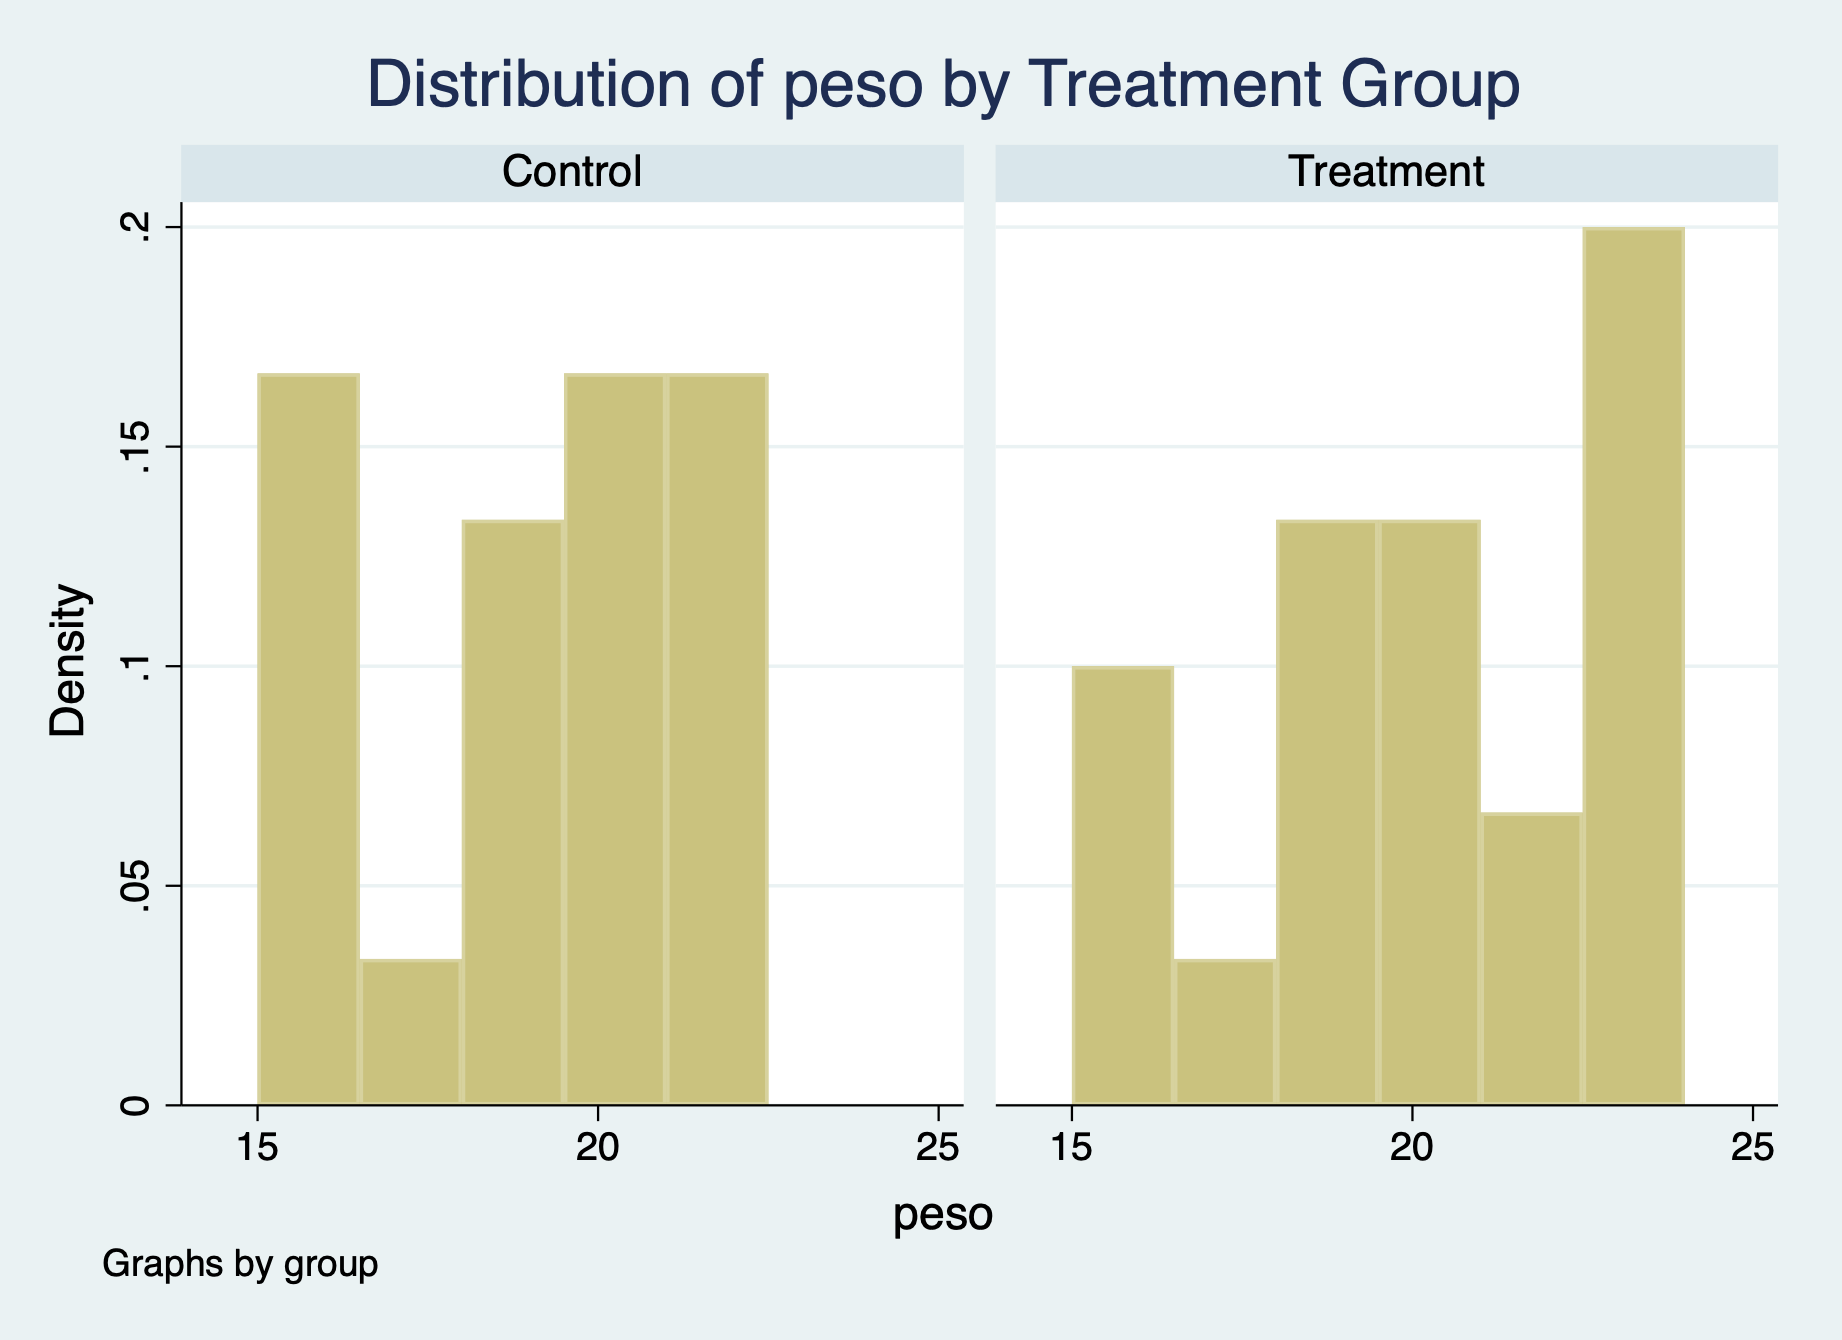
\includegraphics[scale=0.30]{histogram_peso_ntrad.png}
\caption{Histogram of age by Treatment Group}
\end{figure}

\begin{figure}[h]
\centering
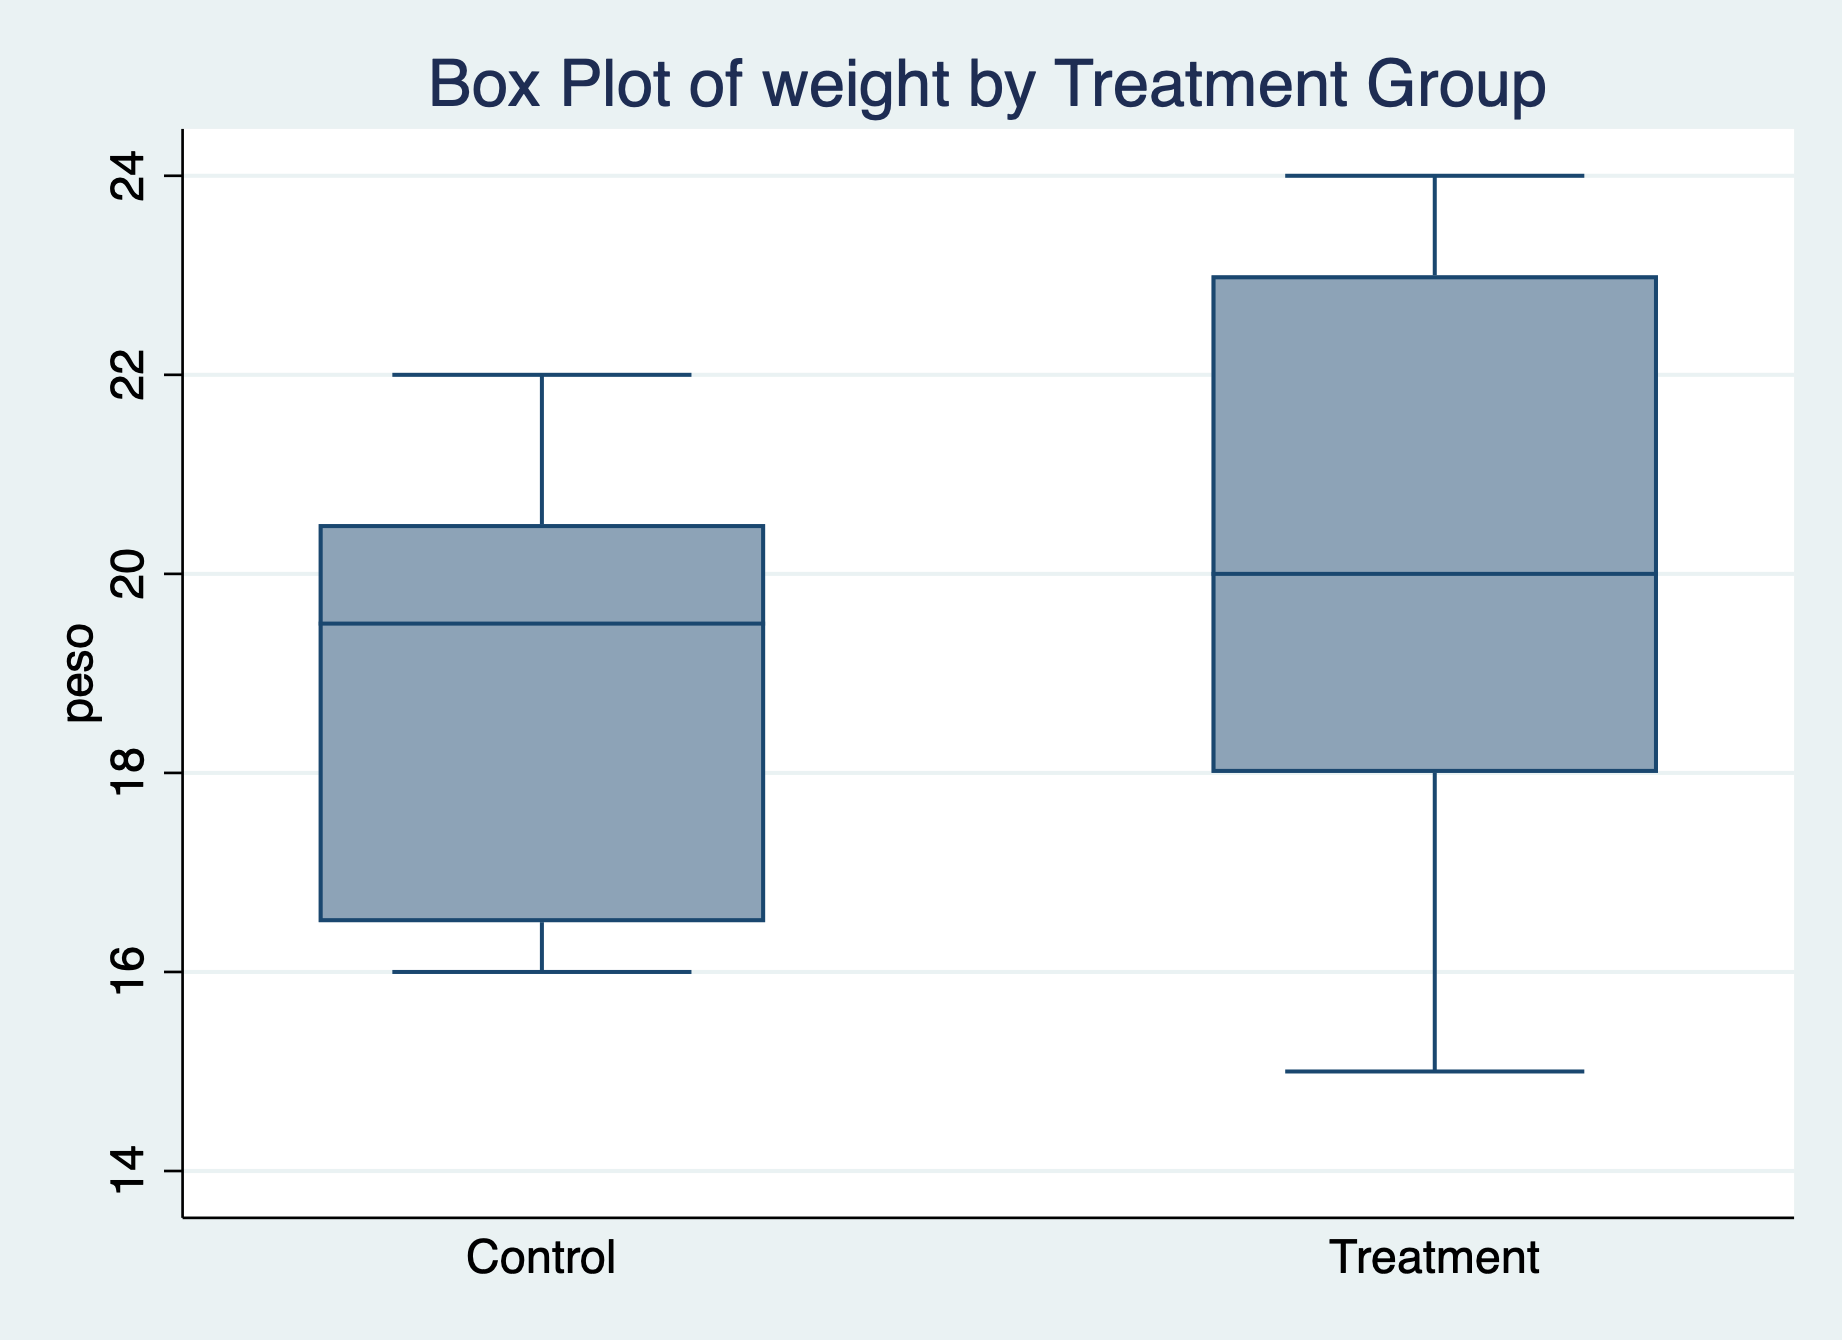
\includegraphics[scale=0.30]{box_plot_peso_ntrad.png}
\caption{Box Plot of age by Treatment Group}
\end{figure}
These graphical representations offer valuable insights into the distribution of key variables between the control
(Metadone) and treatment (Maropitant) groups. Remarkably, the plots depict a high degree of similarity in the
distribution patterns of these variables across both groups. The substantial overlap observed in the plots suggests that
the randomization procedure has achieved a successful balance of covariates between the treatment and control groups.
This harmonious alignment in the plots serves as compelling evidence of the randomization's success, enhancing the
credibility of our experimental findings. It indicates that any observed effects are likely attributable to the
treatment rather than confounding variables, reinforcing the robustness of our conclusions. 
\end{document}
